% Options for packages loaded elsewhere
\PassOptionsToPackage{unicode}{hyperref}
\PassOptionsToPackage{hyphens}{url}
%
\documentclass[
  11pt,
]{article}
\usepackage{amsmath,amssymb}
\usepackage{lmodern}
\usepackage{iftex}
\ifPDFTeX
  \usepackage[T1]{fontenc}
  \usepackage[utf8]{inputenc}
  \usepackage{textcomp} % provide euro and other symbols
\else % if luatex or xetex
  \usepackage{unicode-math}
  \defaultfontfeatures{Scale=MatchLowercase}
  \defaultfontfeatures[\rmfamily]{Ligatures=TeX,Scale=1}
\fi
% Use upquote if available, for straight quotes in verbatim environments
\IfFileExists{upquote.sty}{\usepackage{upquote}}{}
\IfFileExists{microtype.sty}{% use microtype if available
  \usepackage[]{microtype}
  \UseMicrotypeSet[protrusion]{basicmath} % disable protrusion for tt fonts
}{}
\makeatletter
\@ifundefined{KOMAClassName}{% if non-KOMA class
  \IfFileExists{parskip.sty}{%
    \usepackage{parskip}
  }{% else
    \setlength{\parindent}{0pt}
    \setlength{\parskip}{6pt plus 2pt minus 1pt}}
}{% if KOMA class
  \KOMAoptions{parskip=half}}
\makeatother
\usepackage{xcolor}
\usepackage[margin=1in]{geometry}
\usepackage{graphicx}
\makeatletter
\def\maxwidth{\ifdim\Gin@nat@width>\linewidth\linewidth\else\Gin@nat@width\fi}
\def\maxheight{\ifdim\Gin@nat@height>\textheight\textheight\else\Gin@nat@height\fi}
\makeatother
% Scale images if necessary, so that they will not overflow the page
% margins by default, and it is still possible to overwrite the defaults
% using explicit options in \includegraphics[width, height, ...]{}
\setkeys{Gin}{width=\maxwidth,height=\maxheight,keepaspectratio}
% Set default figure placement to htbp
\makeatletter
\def\fps@figure{htbp}
\makeatother
\setlength{\emergencystretch}{3em} % prevent overfull lines
\providecommand{\tightlist}{%
  \setlength{\itemsep}{0pt}\setlength{\parskip}{0pt}}
\setcounter{secnumdepth}{-\maxdimen} % remove section numbering
\usepackage{fancyhdr}
\usepackage{fontspec}
\usepackage{xcolor}
\usepackage{hyperref}
\usepackage{pdfcomment}
\usepackage{datetime}
\usepackage{subfig}
\usepackage{float}
\usepackage[document]{ragged2e}

\setmainfont{Poppins}

% \fancypagestyle{plain}{\pagestyle{fancy}} % added to show header and footer in the first page

% header and footer
\pagestyle{fancy}
\setlength{\headheight}{75pt}
\setlength{\textheight}{600pt}
\fancyhead[C]{}
\fancyhead[L]{\includegraphics{X:/DSA/Trends/household-travel-survey/headers/PST_2021_HTS_header.png}}
\fancyhead[R]{}
\newdateformat{monthyeardate}{\monthname[\THEMONTH] \THEYEAR}
\fancyfoot[L]{\scriptsize{1011 Western Ave, Suite 500, Seattle WA 98104} \textcolor[HTML]{F05A28}. 206.464.7532 \textcolor[HTML]{F05A28}. www.psrc.org \textcolor[HTML]{F05A28}. \monthyeardate\today}
\fancyfoot[R]{\textcolor[HTML]{F05A28}\thepage}
\fancyfoot[C]{}
\renewcommand{\headrulewidth}{0pt}
\renewcommand{\footrulewidth}{4pt}
\renewcommand{\footrule}{\hbox to \headwidth{\color[HTML]{BCBEC0}\leaders\hrule height \footrulewidth\hfill}}
\ifLuaTeX
  \usepackage{selnolig}  % disable illegal ligatures
\fi
\IfFileExists{bookmark.sty}{\usepackage{bookmark}}{\usepackage{hyperref}}
\IfFileExists{xurl.sty}{\usepackage{xurl}}{} % add URL line breaks if available
\urlstyle{same} % disable monospaced font for URLs
\hypersetup{
  pdfauthor={Meg Grzybowski},
  hidelinks,
  pdfcreator={LaTeX via pandoc}}

\author{Meg Grzybowski}
\date{2023-3-7}

\begin{document}

\setmainfont{Poppins}

\floatsetup[figure]{capposition=top}

\hypertarget{delivery-trends-for-the-puget-sound-region}{%
\section{Delivery Trends for The Puget Sound
Region}\label{delivery-trends-for-the-puget-sound-region}}

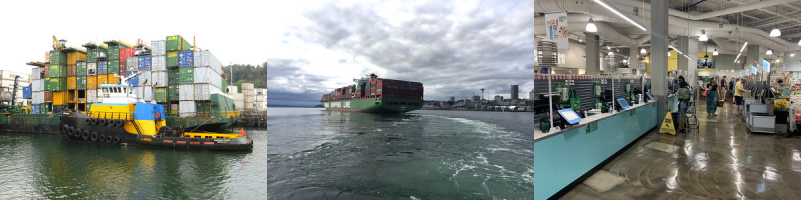
\includegraphics[width=1\textwidth,height=\textheight]{C:/Coding/CURRENT_REPOS_GITHUB/travel-studies/2021/analysis_in_progress/deliveries/trend_story_template/trend_image_header.png}

\begin{flushleft}
The 2021 regional travel survey collected day-to-day information from households in the central Puget Sound region: how we traveled, where we went, how long it took - even where we chose to live and whether we got home deliveries. This report compares household delivery choices in 2021, during COVID-19 conditions, to that in the previous years of 2017 and 2019. Learn more at the \href{https://www.psrc.org/our-work/household-travel-survey-program}{\underline{\textcolor{blue}{PSRC household travel survey webpage}}}. You can also \href{https://household-travel-survey-psregcncl.hub.arcgis.com}{\underline{\textcolor{blue}{view the full travel survey dataset here}}}, including 2017, 2019, and 2021 data.

In some analysis 2017 and 2019 survey samples have been combined to strengthen the statistical validity of the findings by increasing the number of respondents included in the analysis.
\end{flushleft}

\hypertarget{trends-in-home-delivery-and-services}{%
\subsection{Trends in Home Delivery and
Services}\label{trends-in-home-delivery-and-services}}

\begin{flushleft}
One of the questions that the Household Travel Survey QUestionnaire focused on was the frequency of deliveries or services that households received on an average day. The deliveries or services were divided into four major groupings; food or meal delivery (i.e., pizza, prepared meals, Grubhub), grocery delivery (i.e., Amazon Fresh, Instacart, Safeway online), package delivery (i.e., FedEx, UPS, USPS package), or at-home services (i.e., landscaping, cable service, house-cleaning). Across the three data sets (2017, 2019, and 2021), food and grocery deliveries \textbf{more than doubled} from 2019 to 2021 (although, these types of deliveries still only represent a small percentage of households at about 5\%). Package deliveries had a growth rate that doubled between 2019 to 2021. Package deliveries also represent the highest share of delivery types on a average weekday for households. Work or service deliveries remained consistent at around 5\% (Figure 1).
\end{flushleft}

\begin{figure}[H]
\subfloat[Food or Meal\label{fig:individual delivery type-1}]{\includegraphics[width=0.5\linewidth]{delivery_trends_files/figure-latex/individual delivery type-1} }\subfloat[Grocery\label{fig:individual delivery type-2}]{\includegraphics[width=0.5\linewidth]{delivery_trends_files/figure-latex/individual delivery type-2} }\newline\subfloat[Package\label{fig:individual delivery type-3}]{\includegraphics[width=0.5\linewidth]{delivery_trends_files/figure-latex/individual delivery type-3} }\subfloat[Work or Service\label{fig:individual delivery type-4}]{\includegraphics[width=0.5\linewidth]{delivery_trends_files/figure-latex/individual delivery type-4} }\caption{Trends in Home Delivery Types (Source: PSRC Household Travel Survey (2017, 2019, 2021))}\label{fig:individual delivery type}
\end{figure}

\newpage
\setlength{\headheight}{10pt}
\setlength{\textheight}{665pt}
\fancyhead[L]{}

\begin{flushleft} 
As previously seen, package deliveries represent the highest share of home delivery types, and when combined on a fixed scale, it's easy to see the distribution of home delivery or service types (Figure 2). 
\end{flushleft}

\begin{figure}
\centering
\includegraphics{delivery_trends_files/figure-latex/deliveries-1.pdf}
\caption{Trends in Home Deliveries or Services (Source: PSRC Household
Travel Survey (2017, 2019, 2021))}
\end{figure}

\hypertarget{how-income-impacted-food-and-package-deliveries}{%
\subsection{How Income Impacted Food and Package
Deliveries}\label{how-income-impacted-food-and-package-deliveries}}

\begin{flushleft}
Higher income households (over \textdollar 75,000) were \textbf{substantially more likely} to get a food or meal delivery, as compared to lower income households in 2021, but not in previous years. These food or meal deliveries \textbf{more than tripled} between 2021 and previous years (from 1.5\% to 5.5\%). On the flip side, while both lower income and higher income-bracket households had an increase in package deliveries, those households receiving less than \textdollar 75,000 had a significant spike in package deliveries, growing from about 18\% to over 30\% in 2021 (Figure 3).
\end{flushleft}

\begin{figure}[H]
\subfloat[Food or Meal\label{fig:income blocks-1}]{\includegraphics[width=0.5\linewidth]{delivery_trends_files/figure-latex/income blocks-1} }\subfloat[Package\label{fig:income blocks-2}]{\includegraphics[width=0.5\linewidth]{delivery_trends_files/figure-latex/income blocks-2} }\caption{Types of Delivery by Income (Source: Source: PSRC Household Travel Survey (2017, 2019, 2021))}\label{fig:income blocks}
\end{figure}

\hypertarget{households-with-children-received-the-most-packages-in-2021.}{%
\subsection{Households with Children Received the Most Packages in
2021.}\label{households-with-children-received-the-most-packages-in-2021.}}

\begin{flushleft}
Food or meal, grocery, and work or service deliveries stayed relatively stable regardless of household composition
or year. However, package deliveries were the highest for households with kids (45\%), and then decreased as household age increased (about 30\%).
\end{flushleft}

\begin{figure}
\centering
\includegraphics{delivery_trends_files/figure-latex/lifecycle-1.pdf}
\caption{Types of Delivery based on Age Group and Lifecycle Stage
(Source: Source: PSRC Household Travel Survey (2017, 2019, 2021))}
\end{figure}

\hypertarget{food-and-grocery-deliveries-doubled-outside-of-rgcs-in-2021.}{%
\subsection{Food and Grocery Deliveries Doubled Outside of RGCs in
2021.}\label{food-and-grocery-deliveries-doubled-outside-of-rgcs-in-2021.}}

\begin{flushleft}
Since the early 1990s, the central Puget Sound region has adopted a strategy that focus future population and employment growth in designated \href{https://www.psrc.org/our-work/centers}{centers} within the region's urban growth area. Currently, there are 29 dense, walkable, mixed-used areas called  \textbf{regional growth centers (RGCs)}. RGCs are places that higher density and population and employment growth is planned. Based on the most recent findings in 2016, RGCs constitute only 1\% of the region's land area, but contain 5\% share of population and 28\% of employment, as well as 7\% of population growth and 12\% of employment growth. The main function of RGCs is to accommodate significant population and employment growth, as well as to focus regional's investments on housing, services and public transportation to accommodate the large demand that comes with the projected growth. Typically, RGCs are also located in closer proximity to amenities, shops, and resources that, we speculate, typically diminish the need to have deliveries made.

Here we can see that in 2021, the average food/meal or grocery delivery share more than doubled in households
outside of the Regional Growth Centers (RGCs) from nearly 2\% to over 4\%.
\end{flushleft}

\begin{figure}[H]
\subfloat[Food or Meal\label{fig:rgc-1}]{\includegraphics[width=0.5\linewidth]{delivery_trends_files/figure-latex/rgc-1} }\subfloat[Grocery\label{fig:rgc-2}]{\includegraphics[width=0.5\linewidth]{delivery_trends_files/figure-latex/rgc-2} }\caption{Types of Food or Grocery Deliveries by Household Location (Source: Source: PSRC Household Travel Survey (2017, 2019, 2021))}\label{fig:rgc}
\end{figure}

\begin{flushleft}
Package deliveries increased for both RGC and non-RGC households, but package deliveries increased
more significantly in RGCs, from less than 20\% in 2017 and 2019 to almost 20\% in 2021.

Work or service deliveries remained relatively stable from 2017 and 2019 to 2021 in both RGCs and non-RGC households, 
although non-RGC households tended to receive more average work or service deliveries than RGC households.
\end{flushleft}

\includegraphics{delivery_trends_files/figure-latex/unnamed-chunk-1-1.pdf}

\hypertarget{household-deliveries-and-household-size}{%
\subsection{Household Deliveries and Household
Size}\label{household-deliveries-and-household-size}}

\begin{flushleft}
Still interpreting data here.
\end{flushleft}

\begin{figure}[H]
\subfloat[Food or Meal\label{fig:hhsize-1}]{\includegraphics[width=0.5\linewidth]{delivery_trends_files/figure-latex/hhsize-1} }\subfloat[Grocery\label{fig:hhsize-2}]{\includegraphics[width=0.5\linewidth]{delivery_trends_files/figure-latex/hhsize-2} }\newline\subfloat[Package\label{fig:hhsize-3}]{\includegraphics[width=0.5\linewidth]{delivery_trends_files/figure-latex/hhsize-3} }\subfloat[Work or Service\label{fig:hhsize-4}]{\includegraphics[width=0.5\linewidth]{delivery_trends_files/figure-latex/hhsize-4} }\caption{Types of Delivery by Household Size (Source: Source: PSRC Household Travel Survey (2017, 2019, 2021))}\label{fig:hhsize}
\end{figure}

\hypertarget{conclusion}{%
\subsection{Conclusion}\label{conclusion}}

\begin{flushleft}
With increased emotional labor and care-taking demands, and with women more likely to live in poverty and having less employment and lower incomes than men, there are many aspects of transit and transportation modalities that need to be reassessed to support women's needs. Women of color need a robust transit network with more reliable service throughout the day. Biking, walking, and transit don't always feel accessible or safe, and access to a vehicle isn't always available to women. While an increase in telework has removed some of the additional burden to trip-chaining for women, we need to consider how we create and manage transportation so that it may be equitable to all. Transit especially needs to be designed around women of color, since they use transit more than other groups.

While we are working towards a more non-binary understanding of gendered data, we acknowledge that much of the data presented above does analyze information and patterns in a binary manner.

Download the data used in this Trend.
\end{flushleft}

\end{document}
